%!TEX ROOT=../diploma-thesis.tex

\chapter{Anal\'yza problematiky}\label{ch:analyza}

Tato kapitola analyzuje problematiku byznysov\'ych pravidel v informačn\'{\i}ch systémech
a detailně popisuje architekturu orientovanou na služby, včetně jej\'{\i}ho historického
v\'yvoje a modern\'{\i}ch trendů. Na základě toho kapitola popisuje nedostatky
současn\'ych př\'{\i}stupů při sdílení byznysových pravidel. V závěru kapitoly jsou
identifikovány požadavky, které by měl splňovat framework, jež bude v\'ystupem této diplomové práce.

\section{Byznysová pravidla}\label{sec:business-rules}

Podnikové informačn\'{\i} systémy (\gls{EIS} z anglického \textit{Enterprise Information System})
maj\'{\i} za úkol ulehčit, automatizovat či poskytovat podporu pro byznysové procesy organizace,
která je využívá~\cite{dumas2005process}. K tomuto účelu uchovávají a spravují data a měly by zaručit,
že nedojde k jejich poškozen\'{\i} či narušen\'{\i} jejich integrity. Byznysové operace proto
podléhají byznysov\'ym pravidlům, která zajišťuj\'{\i} konzistenci dat informačn\'{\i}ho systému a
zabraňuj\'{\i} nepovolen\'ym operac\'{\i}m~\cite{cemus2015automated}.

\begin{definition}
    Byznysové pravidlo je výraz, který definuje či omezuje některý z byznysových aspektů.
    Jeho úkolem je ověřovat byznysovou strukturu nebo ovlivňovat byznysové chování~\cite{morgan2002business}.
\end{definition}

%Většina stávajících \gls{EIS} využívá tř\'{\i}vrstvou architekturu~\cite{fowler2002patterns}
%rozděluj\'{\i}c\'{\i} systém na datovou vrstvu, aplikačn\'{\i} vrstvu
%a prezentačn\'{\i} vrstvu. Každá z vrstev realizuje jinou funkcionalitu a vzájemně komunikují
%porstřednictvím jasně definovaného rozhraní. Tím se zjednodušuje vývoj a testování systému.
%Byznysová logika je zachycena v aplikační vrstvě, ale byznysová pravidla je potřeba
%zohledňovat ve všech vrstvách systému~\cite{cerny2011reduce}\cite{cemus2015automated}.

\gls{EIS} obsahují mnoho byznysových pravidel, typicky stovky či tisíce~\cite{morgan2002business}.
Samotné pravidlo však bývá relativně krátké a lze shrnout do jedné věty. Díky tomu je pochopitelné
pro všechny zainteresované strany, které se podílejí na návrhu a vývoji systému.
Byznysová pravidla jsou dělena do tř\'{\i} skupin~\cite{cemus2014aspect}:

\begin{description}
    \item [Bezkontextová pravidla] jsou validačn\'{\i} pravidla, která musej\'{\i} b\'yt obecně platná
    v každé byznysové operaci, jinak by mohlo doj\'{\i}t k porušen\'{\i} integrity dat systému.
    \item Př\'{\i}kladem může b\'yt pravidlo \uv{\textit{Adresa uživatele je platnou e-mailovou adresou}}.
    \item [Kontextová pravidla] jsou pravidla, která musej\'{\i} b\'yt zohledněna v daném kontextu
    byznysové operace, např\'{\i}klad \uv{\textit{Při přidán\'{\i} produktu do koš\'{\i}ku nesm\'{\i} součet položek
    v koš\'{\i}ku přesahovat částku milion korun}}
    \item [Průřezová pravidla] jsou parametrizována stavem systému nebo uživatelského účtu a maj\'{\i}
    dopad na velkou část byznysov\'ych operac\'{\i}, například pravidlo \uv{\textit{V systému nesm\'{\i} prob\'{\i}hat
    žádné změny po dobu účetn\'{\i} uzávěrky}}.
\end{description}

Pravidla lze také rozdělit do dvou skupin podle jejich vztahu k byznysové operaci, a těmi jsou
\textit{preconditions} a \textit{post-conditions}~\cite{cemus2015automated}.

\subsection{Precondition}

Aby mohla b\'yt byznysová operace vykonána, musej\'{\i}
b\'yt splněny předem definované podm\'{\i}nky, neboli předpoklady,
které naz\'yváme \textit{preconditions}. Pokud alespoň jedna z podm\'{\i}nek
nen\'{\i} splněna, byznysová operace nemůže proběhnout~\cite{larman2001patterns}.
Například při registraci uživatele mus\'{\i} b\'yt splněna podm\'{\i}nka,
že uživatel vyplnil svoj\'{\i} emailovou adresu, a zároveň
dosud v systému neexistuje žádn\'y uživatel se stejnou emailovou adresou.

\subsection{Post-condition}

Na byznysovou operaci mohou b\'yt kladeny požadavky, které
musej\'{\i} b\'yt splněny po jej\'{\i}m úspěšném vykonán\'{\i}~\cite{cemus2015automated}.
Př\'{\i}kladem může b\'yt anonymizace uživatelů při vytvářen\'{\i} statistického
reportu e-commerce společnosti -- vygenerováný report
nesmí obsahovat citlivé údaje. Dalš\'{\i}m př\'{\i}padem může b\'yt filtrován\'{\i}
v\'ystupu byznysové operace, např\'{\i}klad při v\'ypisu objednávek pro zákazn\'{\i}ka
musí všechny vypsané objednávky patřit danému zákazn\'{\i}kovi.

\subsection{Byznysov\'y kontext}

Informačn\'{\i} systém zpravidla implementuje v\'{\i}ce byznysov\'ych procesů, které se vážou
na jeden či v\'{\i}ce uživatelsk\'ych scénářů~\cite{larman2001patterns}. Uživatelsk\'y scénář se
pak děl\'{\i} na jednotlivé kroky, např\'{\i}klad zaslán\'{\i} potvrzovac\'{\i}ho e-mailu k objednávce, či uložen\'{\i} objednávky
do databáze. Tyto kroky naz\'yváme \textit{byznysové operace} -- tedy operace, které maj\'{\i}
byznysovou hodnotu.

Jak již bylo uvedeno, vykonávání byznysové operace je podmíněno byznysovými pravidly, která se k ní vztahují. Před spuštěním operace musejí
být splněny všechny preconditions, jinak není možné operaci vykonat. Po jejím dokončení musejí být splněny všechny post-conditions.
Aby \gls{EIS} mohl tyto podmínky ověřit dynamicky za běhu systému, využívá tzv. \textit{exekuční kontext} (z anglického
\textit{execution context}), který se skládá z několika dílčích kontextů~\cite{cemus2017separation}:

\begin{description}
    \item[Aplikační kontext] drží stav globáln\'{\i}ch proměnn\'ych systému, jako například nastaven\'{\i}
    produkčn\'{\i}ho režimu, nebo př\'{\i}znak o tom, zda právě prob\'{\i}há obchodn\'{\i} uzávěrka.
    \item[Uživatelský kontext] obsahuje informace o aktuálně přihlášeném uživateli.
    \item[Kontext požadavku] (z anglického \textit{Request context}) se váže zejména na webové služby a obsahuje
    informace o aktuáln\'{\i}m požadavku, jako IP adresa uživatele či jeho geolokace.
    \item[Byznysov\'y kontext] obsahuje informace o probíhající byznysové operaci včetně byznysových pravidel.
\end{description}

Byznysový kontext je tedy důležitým prvkem při výkonu byznysové operace, který umožňuje vyhodnocování byznysových pravidel.
Všechny proměnné, které jsou dostupné v exekučním kontextu, jsou dostupné při vyhodnocování pravidel. Díky tomu je možné
definovat široké spektrum podmínek, které se mohou přizpůsobit aktuálnímu stavu systému.

\begin{definition}
    Byznysový kontext je množina preconditions a post-conditions s byznysovou hodnotou, která se váže na
    konkrétn\'{\i} byznysovou operaci~\cite{cemus2015automated}
\end{definition}

\subsection{Reprezentace byznysového pravidla}

Existuje několik možnost\'{\i}, jak v rámci \gls{EIS} zachytit a reprezentovat byznysová
pravidla~\cite{cemus2015automated}. Těmi jsou:

\benum[label=\circledAlph]
    \item\label{itm:gpl} Zápis v obecném programovacím jazyce
    \item\label{itm:meta} Zápis pomocí meta-instrukcí
    \item\label{itm:dsl} Zápis pomocí doménově specifických jazyků
\eenum

\ref{itm:gpl} je nejběžnějš\'{\i} metodou, umožňující použití stejného jazyka pro popis byznysových pravidel jako
pro popis ostatních částí systému. Bohužel, tato metoda nepřináší možnosti inspekce a extrakce pravidel pro jejich další využití.
\ref{itm:meta} je pokročilejš\'{\i} metodou, která může využívat např\'{\i}klad anotac\'{\i}, nebo tzv. \textit{Expression
Language}~\cite{nemuraite2008representation}. Tato metoda poskytuje dobrou možnost inspekce, ale zpravidla nen\'{\i} typově bezpečná.
Navíc je potřeba meta-instrukce vázat na existující prvky systému, což může být pro některé případy použití omezující~\cite{cemus2015automated}.

\ref{itm:dsl} je nejpokročilejš\'{\i} metodou. \gls{DSL} jsou snadno srozumitelné nejen pro programátory, ale i pro doménové experty.
Navíc mohou b\'yt typově bezpečné. Mezi jejich nev\'yhody ale patř\'{\i} vysoká počátečn\'{\i} investice v podobě návrhu jazyka, nutnosti
jeho kompilace nebo interpretace a také proškolení vývojářů, kteří s ním budou pracovat. Kvůli tomu může být vhodné využít
existující řešení~\cite{cemus2015automated}. Tím může být například Object Constraint Language~\cite{warmer1998object},
který je často využívaný ve výzkumu, nebo některé průmyslové řešení, jako je framework Drools\footnote{\url{https://www.drools.org/}},
který je popsaný v sekci~\ref{sec:drools}.

\section{Architektura orientovaná na služby}\label{sec:soa}

\textit{Architektura orientovaná na služby} (\gls{SOA}) je odpovědí na stále se zvyšující
nároky na informační systémy a jejich rostoucí velikost. Na rozd\'{\i}l od \textit{monolitické architektury},
děl\'{\i} \gls{SOA} systém na samostatné nezávislé celky, zvané \textit{služby}, které jsou
poskytují d\'{\i}lč\'{\i} části požadované funkcionality systému.
Historicky byl term\'{\i}n \gls{SOA} vykládán několika způsoby a představoval
několik rozd\'{\i}ln\'ych, nekompatibiln\'{\i}ch konceptů~\cite{fowler2005serviceorientedambiguity}.
Absence kvalitn\'{\i}ch definic služby a obecně \gls{SOA} vedla k v posledn\'{\i} době i ke snahám
o opuštěn\'{\i} tohoto konceptu~\cite{cerny2017disambiguation}.
Pro lepší porozumění se tato kapitola věnuje stručnému historickému přehledu \gls{SOA}
a shrnuje výhody a nevýhody jednotlivých přístupů.

\begin{definition}
    Služba je znovupoužitelný, soudržný, spravovatelný, nasaditelný a nezávislý proces komunikující
    pomocí zpráv~\cite{papazoglou2003service}\cite{dragoni2017microservices}.
\end{definition}

\subsection{Common Object Request Broker Architecture}\label{sec:corba}

Prvn\'{\i}m historick\'ym předchůdcem architektury orientované na služby
byla tzv. \textit{Common Object Request Broker Architecture}
(\gls{CORBA})~\cite{siegel2000corba}. Ta umožňuje vzájemnou komunikaci aplikací
implementovan\'ych v různ\'ych technologi\'{\i}ch. Její základní komponentou je
je \textit{Object Request Broker} (\gls{ORB}), kter\'y emuluje objekty,
na kter\'ych může klient volat jejich metody. Při zavolán\'{\i} metody
na objektu, kter\'y se fyzicky nacház\'{\i} na vzdáleném stroji,
zprostředkovává \gls{ORB} veškerou komunikaci a poskytuje kompletn\'{\i} rozhran\'{\i}
volaného objektu. Komunikace se vzdálen\'ym objektem s sebou však nese celou řadu problémů,
např\'{\i}klad vyšš\'{\i} latenci při komunikaci nebo v\'yjimečné stavy, které je potřeba
ošetřit, či obížnou optimalizaci kódu využívající \gls{ORB}.

\subsection{Web Services}

Nedostatky architektury \gls{CORBA} vedly k vývoji jednodušš\'{\i}ho
a kvalitnějšího formátu pro popis komunikace služeb. Volán\'{\i} metod na vzdálen\'ych objektech
bylo nahrazeno explicitn\'{\i}m pos\'{\i}lán\'{\i}m zpráv mezi službami pomocí protokolu \gls{HTTP}.
Pro popis schématu zpráv vznikl formát \textit{Simple Object Access
Protocol}~\cite{box2000simple}, kter\'y v kombinaci s
\textit{Web Service Description Language}~\cite{christensen2001web}
umožňuje kompletn\'{\i} definici rozhran\'{\i} pro komunikaci mezi službami.

\subsection{Message Queue}

%\begin{figure}
%    \centering
%    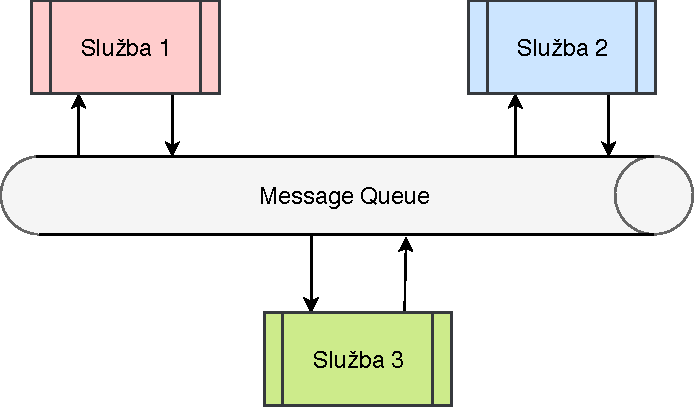
\includegraphics[keepaspectratio=true, width=0.5\linewidth]{figures/message-queue.pdf}
%    \caption{Komunikace služeb pomoc\'{\i} Message Queue}
%    \label{fig:message-queue}
%\end{figure}

Dalš\'{\i}m z konceptů, kter\'y v rámci \gls{SOA} vznikl, je tzv. \textit{Message Queue}.
Jeho základn\'{\i} myšlenkou je asynchronn\'{\i} komunikace služeb pomoc\'{\i} zpráv nezávisl\'ych
na platformě. Komunikaci zprostředkovává fronta, která přij\'{\i}má a rozes\'{\i}lá
zprávy mezi službami. To přináš\'{\i} vyšš\'{\i} škálovatelnost a menš\'{\i} provázanost
mezi službami. Všechny služby ale mus\'{\i} použ\'{\i}vat jednotn\'y formát zpráv.

\subsection{Enterprise Service Bus}

Ačkoliv zm\'{\i}něné modely usnadňuj\'{\i} komunikaci služeb a zvyšuj\'{\i} jejich
spolehlivost, integrace služeb může b\'yt obt\'{\i}žná, pokud služby použ\'{\i}vaj\'{\i}
navzájem různé komunikačn\'{\i} protokoly a formáty. Tento problém řeší \textit{Enterprise Service
Bus} (\gls{ESB})~\cite{chappell2004enterprise}, znázorněn\'y na obrázku~\ref{fig:enterprise-service-bus},
kter\'y má za úkol propojit heterogenn\'{\i} služby a sestavit mezi nimi komunikačn\'{\i} kanály.
T\'{\i}m na sebe \gls{ESB} přeb\'{\i}rá zodpovědnost za překlad jednotliv\'ych zpráv a centralizuje
veškerou komunikaci v systému.

\begin{figure}
    \centering
    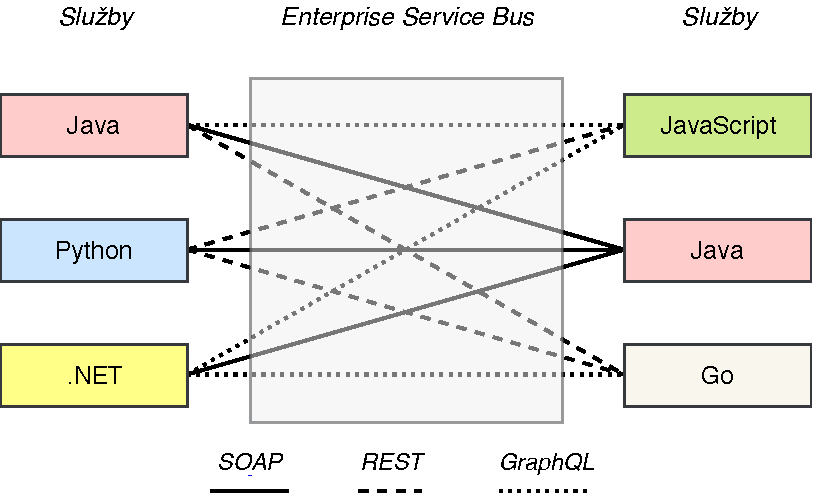
\includegraphics[keepaspectratio=true, width=0.6\linewidth]{figures/enterprise-service-bus.pdf}
    \caption{Komunikace služeb pomocí Enterprise Service Bus}
    \label{fig:enterprise-service-bus}
\end{figure}

\subsection{Microservices}\label{sec:microservices}

%\goal{Microservices a budoucnost SOA}
Microservices je moderní architekturou, která podobně jako \gls{SOA} přináší řešení
problémů pramenících z vysoké komplexity současných \gls{EIS}.
Tato architektura se dá chápat jako podmnožina \gls{SOA}, ačkoliv existují i názory,
že jde o odlišné architektury~\cite{richards2015microservices}\cite{cerny2017disambiguation}.
Vzhledem k její vzrůstající adopci v posledních letech je nutno ji v rámci této práce zohlednit~\cite{xiao2016reflections}.
Základn\'{\i} myšlenkou je v\'yvoj informačn\'{\i}ho systému jako množiny mal\'ych oddělen\'ych služeb,
které jsou spouštěny v samostatn\'ych procesech a komunikuj\'{\i} spolu pomoc\'{\i} jednoduch\'ych
protokolů nezávislých na platformě~\cite{lewis2014microservices}. Microservices preferuje decentralizaci a samostatnost služeb
a zaměřuje se na jejich organizaci kolem byznysov\'ych schopnost\'{\i} systému, nam\'{\i}sto horizontáln\'{\i}ho
dělen\'{\i} systému podle jeho vrstev. Hlavní výhodou tohoto přístupu je flexibilní nasazování a škálování, které je vhodné
pro stále populárnější nasazení v cloudu~\cite{kratzke2017understanding}\cite{cerny2018contextual}\cite{xiao2016reflections}.

\subsection{Orchestrace a choreografie služeb}

Základní podmínkou pro funkci systému stavějícímu na \gls{SOA} je komunikace a spolupráce jednotlivých služeb.
K tomu slouží principy \textit{orchestrace služeb} a \textit{choreografie služeb}.

\paragraph{Orchestrace}
Orchestrace služeb má za úkol zajistit, že komunikace mezi službami
proběhne úspěšně a ve správném časovém sledu~\cite{orchestration},
za použití centráln\'{\i} komponenty -- tzv. \textit{dirigenta}.
Typicky je jako dirigent využ\'{\i}ván \gls{ESB}.

\paragraph{Choreografie}
Př\'{\i}m\'ym opakem orchestrace je tzv. \textit{choreografie služeb} a znamená
vykonáván\'{\i} byznysov\'ych operac\'{\i} autonomně a asynchronně, bez centráln\'{\i}
autority. Tento př\'{\i}stup je preferován zejména v rámci microservices~\cite{dragoni2017microservices},
protože orchestrace vede k vyšš\'{\i}mu provázán\'{\i} služeb a nerovnoměrnému rozložen\'{\i}
zodpovědnost\'{\i} v systémů. Porovnán\'{\i} obou př\'{\i}stupů je graficky
znázorněno na obrázku~\ref{fig:choreography-orchestration}.

\begin{figure}
    \centering
    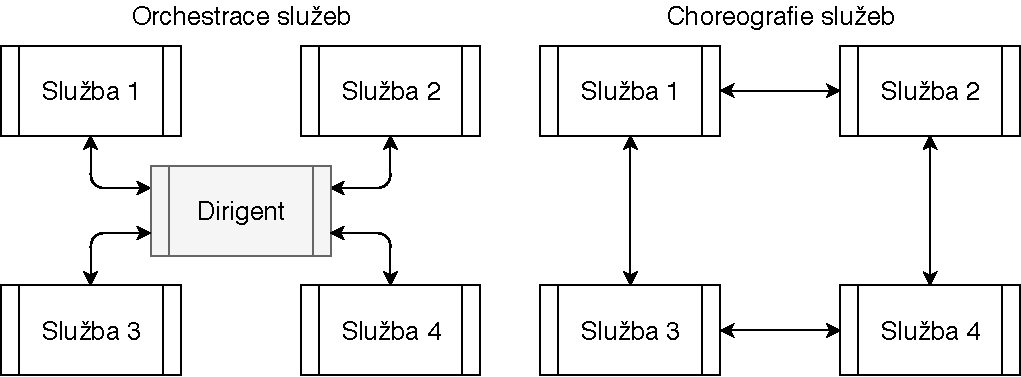
\includegraphics[keepaspectratio=true, width=0.8\linewidth]{figures/choreography-orchestration.pdf}
    \caption{Porovnán\'{\i} orchestrace a choreografie služeb}
    \label{fig:choreography-orchestration}
\end{figure}

\subsection{Shrnutí}

Z předchozího textu vyplývá, že přístupy k realizaci \gls{SOA} vychází ze společné
myšlenky členění systémů do dílčích izolovaných služeb poskytujících byznysovou funkcionalitu.
Přístupy se liší zejména v řešení komunikace služeb a v centralizaci jejich správy.
Historické přístupy využívají komplexní komunikační technologie a umožňují centrální
správu systému, zatímco moderní přístupy od těchto vlastností upouštění. To přináší výzvu
při sdílení byznysových pravidel, která je rozebrána v následující sekci.

\begin{definition}
    \gls{SOA} je soubor návrhových principů, který organizuje komponenty software
    kolem byznysové funkcionality a spojuje je pomocí rozhraní a komunikačních protokolů.
    Každá komponenta je soběstačná a izolovaná, okolnímu světu poskytuje pouze
    své rozhraní~\cite{papazoglou2003service}\cite{lewis2014microservices}.
\end{definition}

\section{Nedostatky současného př\'{\i}stupu}\label{sec:shortcomings}

Některá složitější byznysová funkcionalita vyžaduje kompozici více služeb
najednou~\cite{papazoglou2003service}. Kompozitní služby by měly zohlednit
byznysová pravidla služeb, které ke své funkci využívají, aby zabránily
nekonzistentním stavům v systému a zbytečným spouštěním byznysových operací,
jejichž preconditions nejsou splněny~\cite{cerny2017disambiguation}.
To je však s přímým rozporem s požadavkem na nízkou provázanost služeb, které
by neměly vzájemně znát svoji interní strukturu. Tato skutečnost
vede k nutnosti duplikace byznysových pravidel v kompozitních službách~\cite{cerny2016survey}.

\begin{definition}
    Kompozitní služba získává a kombinuje informace a funkce existujících poskytovatelné
    služeb~\cite{papazoglou2003service}.
\end{definition}

%\goal{Nast\'{\i}něn\'{\i} konkrétn\'{\i}ho př\'{\i}kladu}
Pro lepší představu tohoto problému uvažme e-commerce systém
skládaj\'{\i}c\'{\i} se z několika služeb naprogramovan\'ych v různ\'ych technologi\'{\i}ch,
a procesy vytváření faktury a vytváření objednávky, každý z nich implementovaný jinou službou.
Systém navíc obsahuje službu poskytující webové uživatelské rozhraní.
Při vytvářen\'{\i} faktury za objednávku mus\'{\i} b\'yt nejprve zvalidována fakturačn\'{\i} adresa.
Protože by mohla nastat situace, kdy by v př\'{\i}padě nevalidn\'{\i} adresy museli zaměstnanci
společnosti kontaktovat zákazn\'{\i}ka -- pokud vůbec takovou možnost maj\'{\i}
-- musí být adresa validována již při vytvářen\'{\i} objednávky.
V ideáln\'{\i}m př\'{\i}padě by navíc měl zákazn\'{\i}k být upozorněn na nevalidn\'{\i} fakturačn\'{\i}
adresu co nejdříve, ještě před odeslán\'{\i}m objednávkového formuláře, př\'{\i}mo v uživatelském
rozhran\'{\i}~\cite{cemus2017separation}. Pro ilustraci je problém znázorněn na obrázku~\ref{fig:service-cutting},

%\goal{Náročná údržba a reakce na změnu požadavku}
Na příkladu lze pozorovat, že stejná funkcionalita se prom\'{\i}tá
do tř\'{\i} služeb, z nichž každá má zodpovědnost za jiné byznysové operace.
Stejn\'y kód, kter\'y realizuje validaci fakturačn\'{\i} adresy,
mus\'{\i} b\'yt implementován v každé ze zmiňovaných služeb, navíc v různých technologiích.
Pokud by vzešel změnový požadavek na validaci fakturačn\'{\i} adresy, změnu by bylo nutno
provést konzistentně na třech různ\'ych m\'{\i}stech, všechny tři služby znovu
sestavit a nasadit ve správném pořad\'{\i} tak, aby nedošlo k nekonzistení validaci adresy
při provádění jednotlivých byznysových operací. Změny byznysových pravidel se dějí častěji,
než změny kódu a struktury samotných služeb v \gls{SOA}~\cite{rosenberg2005business}.
Pokud je potřeba s každou změnou byznysového pravidla sestavit a nasadit jednu či více služeb,
dramaticky se zvyšuje náročnost na údržbu takového systému.

\begin{figure}
    \centering
    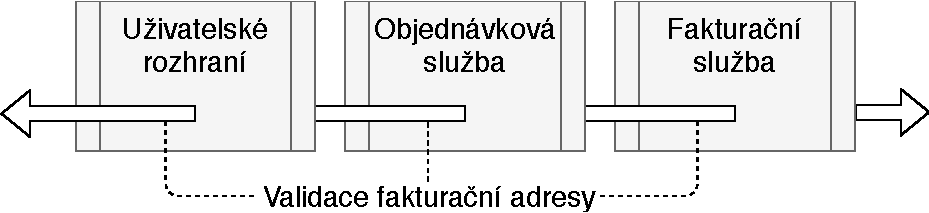
\includegraphics[keepaspectratio=true, width=0.8\linewidth]{figures/service-cutting.pdf}
    \caption{Př\'{\i}klad funkcionality zasahující do v\'{\i}ce služeb}
    \label{fig:service-cutting}
\end{figure}

\section{Identifikace požadavků na implementaci frameworku}\label{sec:implementation-requirements}

Pro usnadnění vývoje a údržby systému stavějícího na \gls{SOA}, který
obsahuje kompozitní služby, je nutné umožnit sdílení byznysových pravidel.
Ta by měla být zachycena mimo samotnou implementaci služby, ideálně ve formátu, který bude nezávislý na
konkrétní platformě, bude poskytovat možnost automatické inspekce a bude srozumitelný doménovým expertům.
Úprava pravidel by navíc neměla vyžadovat změnu kódu služby a její opětovné nasazování.
Administrátoři systému by měly mít možnost byznysová pravidla spravovat centrálně a bez
přerušení provozu systému, aby mohli co nejrychleji a flexibilně reagovat na změnové požadavky.

Framework, který bude výstupem této práce, by tedy měl splňovat následující vlastnosti:

\begin{itemize}
    \item{Možnost definovat byznysová pravidla pomoc\'{\i} platformově nezávislého \gls{DSL} srozumitelného pro doménové experty}
    \item{Možnost centrálně spravovat byznysová pravidla, včetně úpravy stávaj\'{\i}c\'{\i}ch a vytvářen\'{\i} nov\'ych dynamicky za běhu systému}
    \item{Automatická distribuce a integrace byznysových pravidel včetně vyhodnocován\'{\i} preconditions a aplikace post-conditions}
    \item{Možnost využ\'{\i}vat framework na v\'{\i}ce plaformách}
\end{itemize}

\section{Shrnut\'{\i}}

V této kapitole byla provedena analýza byznysov\'ych pravidel a byznysov\'ych kontextů a architektury orientované na služby.
Dále byly popsány nedostatky \gls{SOA} při kompozici služeb a sdílení byznysových pravidel.
Nakonec byly identifikovány požadavky, které by měl splňovat framework, který bude v\'ystupem této práce.
